\documentclass[12pt]{beamer}
\usepackage{../Estilos/BeamerMAF}
\usepackage[absolute, overlay]{textpos}
\usepackage{../Estilos/ColoresLatex}
\usetheme{Copenhagen}
\usecolortheme{wolverine}
%\useoutertheme{default}
\setbeamercovered{invisible}
% or whatever (possibly just delete it)
\setbeamertemplate{section in toc}[sections numbered]
\setbeamertemplate{subsection in toc}[subsections numbered]
\setbeamertemplate{subsection in toc}{\leavevmode\leftskip=3.2em\rlap{\hskip-2em\inserttocsectionnumber.\inserttocsubsectionnumber}\inserttocsubsection\par}
% \setbeamercolor{section in toc}{fg=blue}
% \setbeamercolor{subsection in toc}{fg=blue}
% \setbeamercolor{frametitle}{fg=blue}
\setbeamertemplate{caption}[numbered]

\setbeamertemplate{footline}
\beamertemplatenavigationsymbolsempty
\setbeamertemplate{headline}{}


\makeatletter
% \setbeamercolor{section in foot}{bg=gray!30, fg=black!90!orange}
% \setbeamercolor{subsection in foot}{bg=blue!30}
% \setbeamercolor{date in foot}{bg=black}
\setbeamertemplate{footline}
{
  \leavevmode%
  \hbox{%
  \begin{beamercolorbox}[wd=.333333\paperwidth,ht=2.25ex,dp=1ex,center]{section in foot}%
    \usebeamerfont{section in foot} \insertsection
  \end{beamercolorbox}%
  \begin{beamercolorbox}[wd=.333333\paperwidth,ht=2.25ex,dp=1ex,center]{subsection in foot}%
    \usebeamerfont{subsection in foot}  \insertsubsection
  \end{beamercolorbox}%
  \begin{beamercolorbox}[wd=.333333\paperwidth,ht=2.25ex,dp=1ex,right]{date in head/foot}%
    \usebeamerfont{date in head/foot} \insertshortdate{} \hspace*{2em}
    \insertframenumber{} / \inserttotalframenumber \hspace*{2ex} 
  \end{beamercolorbox}}%
  \vskip0pt%
}
\makeatother

\makeatletter
\patchcmd{\beamer@sectionintoc}{\vskip1.5em}{\vskip0.8em}{}{}
\makeatother

% %\newlength{\depthofsumsign}
% \setlength{\depthofsumsign}{\depthof{$\sum$}}
% \newcommand{\nsum}[1][1.4]{% only for \displaystyle
%     \mathop{%
%         \raisebox
%             {-#1\depthofsumsign+1\depthofsumsign}
%             {\scalebox
%                 {#1}
%                 {$\displaystyle\sum$}%
%             }
%     }
% }
% \def\scaleint#1{\vcenter{\hbox{\scaleto[3ex]{\displaystyle\int}{#1}}}}
% \def\scaleoint#1{\vcenter{\hbox{\scaleto[3ex]{\displaystyle\oint}{#1}}}}
% \def\bs{\mkern-12mu}


\setbeamercolor{section in foot}{bg=peridot, fg=black}
\setbeamercolor{subsection in foot}{bg=powderblue(web), fg=black}


\makeatletter
\setbeamertemplate{footline}
{
\leavevmode%
\hbox{%
\begin{beamercolorbox}[wd=.333333\paperwidth,ht=2.25ex,dp=1ex,center]{section in foot}%
  \usebeamerfont{section in foot} \insertsection
\end{beamercolorbox}%
\begin{beamercolorbox}[wd=.333333\paperwidth,ht=2.25ex,dp=1ex,center]{subsection in foot}%
  \usebeamerfont{subsection in foot}  \insertsubsection
\end{beamercolorbox}%
\begin{beamercolorbox}[wd=.333333\paperwidth,ht=2.25ex,dp=1ex,right]{date in head/foot}%
  \usebeamerfont{date in head/foot} \insertshortdate{} \hspace*{1.5em}
  \insertframenumber{} / \inserttotalframenumber \hspace*{2ex} 
\end{beamercolorbox}}%
\vskip0pt%
}
\makeatother
\usefonttheme{serif}
\setbeamercolor{frametitle}{bg=palecerulean}
\resetcounteronoverlays{saveenumi}

\date{17 de mayo de 2022}

\title{\large{Ecuación radial del átomo de hidrógeno}}
\subtitle{Funciones de Laguerre}
\author{M. en C. Gustavo Contreras Mayén}

\begin{document}
\maketitle
\fontsize{14}{14}\selectfont
\spanishdecimal{.}

\section*{Contenido}
\frame{\frametitle{Temas a revisar} \tableofcontents[currentsection, hideallsubsections]}

\section{Normalización función radial}
\frame{\tableofcontents[currentsection, hideothersubsections]}
\subsection{Marco teórico}

\begin{frame}
\frametitle{Solución completa}
Del estudio de la ecuación del átomo de hidrógeno, se obtuvo la solución general de la ecuación de onda en términos de tres números cuánticos: $n$, $\ell$ y $m$
\begin{align*}
\psi_{n \ell m} (r, \theta, \phi) =  R_{n \ell} (r) Y_{\ell}^{m} (\theta, \phi)
\end{align*}
\end{frame}
\begin{frame}
\frametitle{Solución parte radial}
Donde la parte radial a la solución está dada por:
\begin{align*}
R_{n \ell}(r) = \dfrac{1}{r} \, \rho^{\ell + 1} \, e^{-\rho} \, v(\rho)
\end{align*}
\\
\bigskip
\pause
En particular para $R_{20}$, se tiene que:
\begin{align*}
R_{20}(r) = \dfrac{c_{0}}{2 \, a} \left( 1 - \dfrac{r}{2 \, a} \right) \, e^{-r/2a}
\end{align*}
\end{frame}

%Ref. Griffits (2005) Problem 4.11 (a)
\section{Ejercicio 1}
\frame{\tableofcontents[currentsection, hideothersubsections]}
\subsection{Planteamiento}

\begin{frame}
\frametitle{Enunciado del problema}
Normaliza la función $R_{20}$ para construir la función $\psi_{200}$.
\\
\bigskip
\pause
¿Qué tenemos que hacer? \pause
De la función:
\begin{align*}
R_{20}(r) = \dfrac{c_{0}}{2 \, a} \left( 1 - \dfrac{r}{2 \, a} \right) \, e^{-r/2a}
\end{align*}
Hay que determinar los coeficientes $c_{0}$.
\end{frame}

\subsection{Solución}

\begin{frame}
\frametitle{Punto de partida}
Partimos de la normalización de la función:
\begin{align*}
\scaleint{6ex}_{\bs 0}^{\infty} \abs{R_{20}}^{2} \, r^{2} \dd{r} = 1
\end{align*}
\pause
Por lo que:
\begin{align*}
\scaleint{6ex}_{\bs 0}^{\infty} \abs{ \dfrac{c_{0}}{2 \, a} \left( 1 - \dfrac{r}{2 \, a} \right) \, e^{-r/2a} }^{2} r^{2} \dd{r} = 1
\end{align*}
\end{frame}
\begin{frame}
\frametitle{Desarrollo}
Entonces tenemos que:
\begin{align*}
\scaleint{6ex}_{\bs 0}^{\infty} \left(\dfrac{c_{0}}{2 \, a}\right)^{2} \left( 1 - \dfrac{r}{2 \, a} \right)^{2} \, e^{-r/a} \, r^{2} \dd{r} = 1
\end{align*}
\\
\bigskip
\pause
Para resolver esta integral, \pause proponemos el cambio de variable: $z = \dfrac{r}{a}$
\end{frame}
\begin{frame}
\frametitle{Expresión con el cambio}
\begin{align*}
\scaleint{6ex}_{\bs 0}^{\infty} \bigg( \dfrac{c_{0}}{2 \, a} \bigg)^{2} \, \bigg( 1 - \dfrac{z}{2} \bigg)^{2} \, e^{-z} \, (a \, z)^{2} a \, \dd{z} = 1
\end{align*}
\\
\bigskip
\pause
Que simplificando, obtenemos:
\pause
\begin{align*}
\bigg( \dfrac{c_{0}}{2 \, a} \bigg)^{2} \, a^{3} \, \scaleint{6ex}_{\bs 0}^{\infty} \bigg( 1 - \dfrac{z}{2} \bigg)^{2} \, e^{-z} \, z^{2} \dd{z} = 1
\end{align*}
\end{frame}
\begin{frame}
\frametitle{Resolviendo la integral}
Desarrollando el binomio en el integrando:
\pause
\begin{align*}
\dfrac{c_{0}^{2} \, a}{4} \, \scaleint{6ex}_{\bs 0}^{\infty} \left( 1 - z + \dfrac{z^{2}}{4} \right) \, e^{-z} \, z^{2} \dd{z} = 1
\end{align*}
\pause
Entonces tendremos:
\begin{align*}
\dfrac{c_{0}^{2} \, a}{4} \, \scaleint{6ex}_{\bs 0}^{\infty} \left( z^{2} - z^{3} + \dfrac{z^{2}}{4} \right) \, e^{-z} \dd{z} = 1
\end{align*}
\end{frame}
\begin{frame}
\frametitle{Ocupando un resultado conocido}
Sabemos que una integral del tipo:
\begin{eqnarray*}
\scaleint{6ex}_{\bs 0}^{\infty} z^{n} \, e^{-z} \dd{z} = \pause \Gamma(n + 1) = \pause n!
\end{eqnarray*}
\pause
Por lo que la integral anterior se resuelve en términos del valor del factorial de cada término:
\end{frame}
\begin{frame}
\frametitle{Solución a la integral}
Al resolver la integral de la suma de cada término, tendremos que:
\pause
\begin{equation*}
\begin{aligned}
\dfrac{c_{0}^{2} \, a}{4} \, &\left[ 2 - 6 + \dfrac{24}{4} \right] = 1 \\[0.5em] \pause
\dfrac{a}{2} \, c_{0}^{2} &= 1 \\[0.5em] \pause
\Rightarrow c_{0} &= \sqrt{\dfrac{2}{a}}
\end{aligned}
\end{equation*}
\end{frame}
\begin{frame}
\frametitle{La función radial ya es conocida}
Una vez obtenido el valor de $c_{0}$ ya se puede ocupar para la función radial:
\pause
\begin{align*}
R_{20} (r) = \sqrt{\dfrac{2}{a}} \, \dfrac{1}{2 a} \bigg( 1 - \dfrac{r}{2 a} \bigg) \, e^{-r/2a}
\end{align*}
\end{frame}
\begin{frame}
\frametitle{Gráfica de la función radial}
\begin{figure}
   \centering
   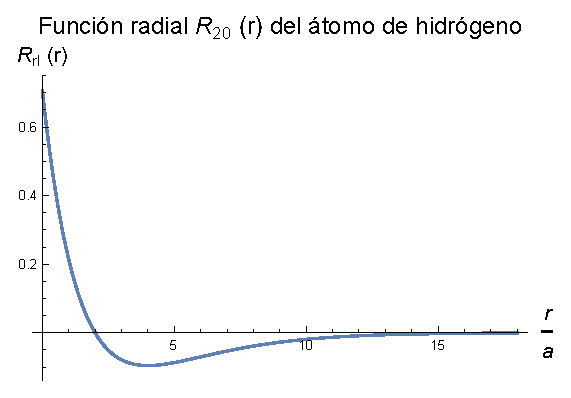
\includegraphics[scale=1]{Imagenes/Plot_Hermite_Radial_20.eps}
\end{figure}
\end{frame}
\begin{frame}
\frametitle{La solución}
La solución general es:
\begin{align*}
\psi_{n \ell m} (r, \theta, \phi) = R_{n \ell} (r) \, Y_{\ell}^{m} \, (\theta, \phi)
\end{align*}
\pause
Lo que nos pide el enunciado es:
\begin{align*}
\psi_{200} = R_{2 0} (r) \, Y_{0}^{0} \, (\theta, \phi)
\end{align*}
\end{frame}
\begin{frame}
\frametitle{Otro resultado conocido}
Como ya conocemos el valor del armónico esférico:
\begin{align*}
Y_{0}^{0} \, (\theta, \phi) = \dfrac{1}{\sqrt{4 \, \pi}}
\end{align*}
\end{frame}
\begin{frame}
\frametitle{Solución al problema}
Juntamos los resultados, para llegar a:
\pause
\begin{eqnarray*}
\begin{aligned}
\psi_{200} &= \dfrac{1}{\sqrt{4 \, \pi}} \, \sqrt{\dfrac{2}{a}} \, \dfrac{1}{2 \, a} \bigg( 1 - \dfrac{r}{2 \, a} \bigg) \, e^{-r/2a} \\[1em] \pause
\psi_{200} &= \dfrac{1}{\sqrt{2 \, \pi \, a}} \, \dfrac{1}{2 \, a} \bigg( 1 - \dfrac{r}{2 \, a} \bigg) \, e^{-r/2a} \qed
\end{aligned}
\end{eqnarray*}
\end{frame}
\begin{frame}
\frametitle{Gráfica en 3D}
Una visualización de la función de onda $\psi_{200}$ se muestra a continuación:
\pause
\begin{figure}
   \centering
   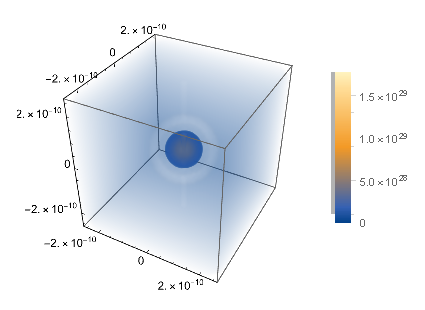
\includegraphics[scale=1]{Imagenes/Plot_Funcion_Onda_200.eps}
\end{figure}
\end{frame}

%Ref. Griffits (2005) Problem 4.11 (b)
\section{Ejercicio 2}
\frame{\tableofcontents[currentsection, hideothersubsections]}
\subsection{Enunciado}

\begin{frame}
\frametitle{Enunciado del ejercicio}
Normaliza la función radial:
\begin{align*}
R_{21} (r) = \dfrac{c_{0}}{4 a^{2}} \, r \, e^{-r/2a}
\end{align*}
\pause
Para construir las funciones de onda: $\psi_{211}, \psi_{210}$ y $\psi_{21-1}$
\end{frame}
\begin{frame}
\frametitle{Nuevamente la normalización}
Para obtener el valor del coeficiente $c_{0}$, debemos de normalizar la función $R_{21} (r)$:
\pause
\begin{align*}
\scaleint{6ex}_{\bs 0}^{\infty} \abs{R_{21}}^{2} \, r^{2} \, \dd{r} = 1
\end{align*}
\end{frame}
\begin{frame}
\frametitle{Expresión a calcular}
Entonces se tiene que:
\pause
\begin{eqnarray*}
\begin{aligned}
&\scaleint{6ex}_{\bs 0}^{\infty} \bigg( \dfrac{c_{0}}{4 a^{2}} \, r \, e^{-r/2a} \bigg)^{2} \, r^{2} \dd{r} = 1 \\[0.5em] \pause
&\dfrac{c_{0}^{2}}{16 a^{4}} \, \scaleint{6ex}_{\bs 0}^{\infty}  r^{4} \, e^{-r/a} \dd{r} = 1
\end{aligned}
\end{eqnarray*}
\end{frame}
\begin{frame}
\frametitle{Hacemos cambio de variable}
Se ocupa el mismo cambio de variable que en el ejercicio anterior, es decir: $z = r/a$:
\pause
\begin{eqnarray*}
\begin{aligned}
&\dfrac{c_{0}^{2} \, a}{16} \, \scaleint{6ex}_{\bs 0}^{\infty}  z^{4} \, e^{-z} \dd{z} = 1 \\[0.5em] \pause
\Rightarrow \hspace{0.2cm} &\dfrac{c_{0}^{2} \, a}{16} \, (4!) = 1 \\[0.5em] \pause
\Rightarrow \hspace{0.2cm} &\dfrac{3 \, c_{0}^{2} \, a}{2} = 1 \pause \hspace{0.5cm} \Rightarrow \hspace{0.2cm} c_{0} = \sqrt{\dfrac{2}{3 \, a}}
\end{aligned}
\end{eqnarray*}
\end{frame}
\begin{frame}
\frametitle{La función radial}
Por lo que la función radial $R_{21} (r)$ es:
\pause
\begin{align*}
R_{21} (r) = \dfrac{1}{\sqrt{6 \, a}} \, \dfrac{1}{2 \, a^{2}} \, r \, e^{-2/ra}
\end{align*}
\end{frame}
\begin{frame}
\frametitle{Gráfica de la función radial}
\begin{figure}
   \centering
   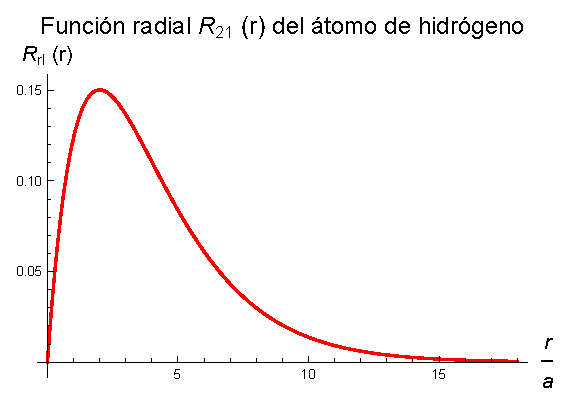
\includegraphics[scale=1]{Imagenes/Plot_Hermite_Radial_21.eps}
\end{figure}
\end{frame}
\begin{frame}
\frametitle{Ocupando los armónicos esféricos}
Para la solución completa, debemos de ocupar los armónicos esféricos:
\pause
\begin{align*}
Y_{1}^{0} (\theta, \phi) = \bigg( \dfrac{3}{4 \, \pi} \bigg)^{\frac{1}{2}} \cos \theta
\end{align*}
\pause
De manera conveniente, tenemos que:
\pause
\begin{align*}
Y_{1}^{\pm 1} (\theta, \phi) = \mp \bigg( \dfrac{3}{8 \, \pi} \bigg)^{\frac{1}{2}} \sin \theta \, e^{\pm i \phi}
\end{align*}
\end{frame}
\begin{frame}
\frametitle{Solución para $\psi_{210}$}
Al juntar los resultados de la parte radial y el correspondiente armónico esférico, la solución es:
\pause
\begin{eqnarray*}
\begin{aligned}
\psi_{210} (r, \theta, \phi) &= \dfrac{1}{\sqrt{6 \, a}} \, \dfrac{1}{2 \, a^{2}} \, r \, e^{-r/2a} \, \sqrt{\dfrac{3}{4 \, \pi}} \cos \theta = \\[0.5em] \pause
&= \dfrac{1}{2 \, \pi \, a} \, \dfrac{1}{4 \, a^{2}} \, r \, e^{-r/2a} \, \cos \theta
\end{aligned}
\end{eqnarray*}
\end{frame}
\begin{frame}
\frametitle{Solución para $\psi_{21 \pm 1}$}
Al juntar ahora los resultados de la parte radial y el correspondiente armónico esférico, cuidando los signos, la solución es:
\pause
\begin{eqnarray*}
\begin{aligned}
\psi_{21 \pm 1} (r, \theta, \phi) &= \dfrac{1}{\sqrt{6 \, a}} \, \dfrac{1}{2 \, a^{2}} \, r \, e^{-r/2a} \times \\[0.5em]
&\times \bigg[ \mp \, \sqrt{\dfrac{3}{8 \, \pi}} \, \sin \theta \, e^{\pm i \phi} \bigg]  =
\end{aligned}
\end{eqnarray*}
\end{frame}
\begin{frame}
\frametitle{Solución para $\psi_{21 \pm 1}$}
La solución simplificada para las funciones radiales es:
\pause
\begin{align*}
\psi_{21 \pm 1} (r, \theta, \phi) = \mp \, \dfrac{1}{\sqrt{\pi \, a}} \, \dfrac{1}{8 \, a^{2}} \, r \, e^{-2/ra} \, \sin \theta \, e^{\pm i \phi}
\end{align*}
\end{frame}
\begin{frame}
\frametitle{Gráfica en 3D}
Una visualización de la función de onda $\psi_{21 \pm 1}$ se muestra a continuación:
\pause
\begin{figure}
   \centering
   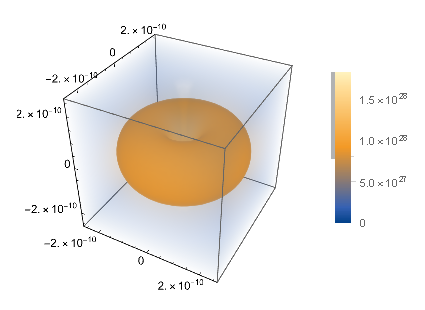
\includegraphics[scale=1]{Imagenes/Plot_Funcion_Onda_211.eps}
\end{figure}
\end{frame}

%Ref. Zettilli (2009) 6.3 (e)
\section{La función radial}
\frame{\tableofcontents[currentsection, hideothersubsections]}
\subsection{Expresión analítica}

\begin{frame}
\frametitle{Las funciones radiales}
En la mecánica cuántica se estudia a profundidad el átomo de hidrógeno.
\\
\bigskip
\pause
Con el desarrollo que se ha hecho sobre la parte radial del problema, es importante también describir el comportamiento de la solución.
\end{frame}
\begin{frame}
\frametitle{La expresión para $R_{n \ell}$}
Se tiene que:
\pause
\begin{align*}
R_{n \ell} (r) &= - \left( \dfrac{2}{n \, a_{0}} \right)^{3/2} \sqrt{\dfrac{(n - 1 -\ell)!}{2 \, n \big[(n + \ell) \big]^{3}}} \, \left( \dfrac{2 \, r}{n \, a_{0}} \right)^{\ell} \times \\[0.5em]
&\times e^{-r/n a_{0}} \, L_{n+\ell}^{2 \ell+1} \left( \dfrac{2 \, r}{n \, a_{0}} \right)
\end{align*}
donde $L_{\ell}^{m}$ es el polinomio asociado de Laguerre de orden $\ell m$, y $a_{0}$ es el radio de Bohr.
\end{frame}
\begin{frame}
\frametitle{Propiedades de las funciones de onda radiales}
\setbeamercolor{item projected}{bg=black,fg=white}
\setbeamertemplate{enumerate items}{%
\usebeamercolor[bg]{item projected}%
\raisebox{1.5pt}{\colorbox{bg}{\color{fg}\footnotesize\insertenumlabel}}%
}
\begin{enumerate}[<+->]
\item Tienen un comportamiento similar a $r^{\ell}$ para valores pequeños de $r$.
\seti
\end{enumerate}
\end{frame}
\begin{frame}
\frametitle{Propiedades de las funciones de onda radiales}
\setbeamercolor{item projected}{bg=black,fg=white}
\setbeamertemplate{enumerate items}{%
\usebeamercolor[bg]{item projected}%
\raisebox{1.5pt}{\colorbox{bg}{\color{fg}\footnotesize\insertenumlabel}}%
}
\begin{enumerate}[<+->]
\conti   
\item Presentan un decaimiento exponencial para valores grandes de $r$, ya que $L_{n+\ell}^{2 \ell+1}$ queda dominado para potencias elevadas de $r^{n-\ell-1}$
\seti
\end{enumerate}
\end{frame}
\begin{frame}
\frametitle{Propiedades de las funciones de onda radiales}
\setbeamercolor{item projected}{bg=black,fg=white}
\setbeamertemplate{enumerate items}{%
\usebeamercolor[bg]{item projected}%
\raisebox{1.5pt}{\colorbox{bg}{\color{fg}\footnotesize\insertenumlabel}}%
}
\begin{enumerate}[<+->]
\conti
\item Cada función $R_{n \ell}(r)$ tiene $n-\ell-1$ nodos radiales, ya que $L_{n+\ell}^{2 \ell+1}(\rho)$ es un polinomio de grado $n - \ell - 1$.
\end{enumerate}
\end{frame}

%Ref. Perez - El  átomo de hidrógeno
\section{Solución átomo de hidrógeno}
\frame{\tableofcontents[currentsection, hideothersubsections]}
\subsection{Expresión}

\begin{frame}
\frametitle{Solución completa}
Se tiene entonces que la solución completa al problema del átomo de hidrógeno en coordenadas esféricas es:
\pause
\begin{align*}
\psi_{n l m} (r, \theta, \phi) &= R_{n \ell}(r) \, Y_{l}^{m} (\theta, \phi) \\[0.5em]
&\begin{cases}
n = & 1, 2, 3 \\
\ell = & 0, 1, 2, \ldots n-1 \\
m &= -\ell, -\ell + 1, \ldots, \ell -1, \ell
\end{cases}
\end{align*}
\end{frame}
\begin{frame}
\frametitle{La función radial}
La función radial está dada por:
\pause
\begin{align*}
R_{n \ell} &= - \bigg( \dfrac{2}{n a_{0}} \bigg)^{\frac{3}{2}} \, \sqrt{\dfrac{(n - \ell - 1)!}{2 n [(n + \ell)]^{3}]}} \, \bigg( \dfrac{2 r}{n a_{0}} \bigg)^{\ell} \times \\[0.5em]
&\times \exp\bigg( - \dfrac{r}{n a_{0}} \bigg) L_{n+\ell}^{2\ell+1} \bigg( \dfrac{2 r}{n a_{0}} \bigg)
\end{align*}
\end{frame}
\begin{frame}
\frametitle{La función angular}
La función radial está dada por los armónicos esféricos:
\pause
\begin{align*}
Y_{\ell}^{m} (\theta, \phi) &= (-1)^{m} \bigg[ \dfrac{(2 \ell + 1)(\ell - \abs{m})!}{4 \pi (\ell + \abs{m})!} \bigg]^{\frac{1}{2}} \times \\[0.5em]
&\times P_{\ell}^{\abs{m}} (\cos \theta) \, e^{i m \phi}
\end{align*}
\end{frame}

\subsection{Estados cuánticos}

\begin{frame}
\frametitle{Estados y números cuánticos}
Las funciones de onda (\emph{orbitales hidrogenoides}) están definidos a partir de los números cuánticos:
\pause
\setbeamercolor{item projected}{bg=black,fg=white}
\setbeamertemplate{enumerate items}{%
\usebeamercolor[bg]{item projected}%
\raisebox{1.5pt}{\colorbox{bg}{\color{fg}\footnotesize\insertenumlabel}}%
}
\begin{enumerate}[<+->]
\item $n$: determina la energía \pause $\to$ número cuántico principal.
\item $l$: determina el módulo del momento angular \pause $\to$ número cuántico angular.
\item $m$: determina la proyección del momento angular en el eje $z$ \pause $\to$ número cuántico azimutal o magnético.
\end{enumerate}
\end{frame}
\begin{frame}
\frametitle{Estados y números cuánticos}
Los correspondientes estados están caracterizados por dichos números cuánticos, por lo que se suelen designar con la notación $\ket{n l m}$.
\end{frame}
\begin{frame}
\frametitle{Notación estado de la función de onda}
Otra notación muy empleada consiste en designar al orbital con el número $n$ seguido de la notación introducida para el armónico esférico.
\end{frame}
\begin{frame}
\frametitle{Notación estado de la función de onda}
Por ejemplo:
\pause
\begin{table}[H]
   \renewcommand{\arraystretch}{1.3}
   \centering
   \begin{tabular}{l l}
      $\ket{100}$ & $1 \, s$ \\ \pause
      $\ket{200}$ & $2 \, s$ \\ \pause
      $\ket{210}$ & $2 \, p_{0}$ \\ \pause
      $\ket{21-1}$ & $2 \, p_{-1}$ \\ \pause
      $\ket{211}$ & $2 \, p_{1}$ \\ \pause
      $\ket{300}$ & $3 \, s$ \\
   \end{tabular}
\end{table}
\end{frame}

\section{Orbitales hidrogenoides}
\frame{\tableofcontents[currentsection, hideothersubsections]}
\subsection{Densidad de distribución radial}

\begin{frame}
\frametitle{Densidad de distribución radial}
Proporciona la densidad de probabilidad de encontrar al electrón a una distancia $r$.
\\
\bigskip
\pause
Se obtiene al integrar $\abs{\psi_{n \ell m} (r, \theta, \phi)}^{2}$ respecto a los ángulos $\theta$ y $\phi$.
\end{frame}
\begin{frame}
\frametitle{Densidad de distribución radial}
Viene dada por la expresión:
\pause
\begin{eqnarray*}
\begin{aligned}
D_{n \ell} (r) &= \scaleint{6ex}_{\bs 0}^{2 \pi} \scaleint{6ex}_{\bs 0}^{\pi} \psi_{n \ell m}^{*} (r, \theta, \phi) \, r^{2} \, \psi_{n \ell m} (r, \theta, \phi) \times \\[0.5em]
&\times\sin \theta \dd{\theta} \dd{\phi} = \\[0.5em] \pause
&= r^{2} \, R_{n \ell} (r)
\end{aligned}
\end{eqnarray*}
\pause
Considerando que los armónicos esféricos están normalizados.
\end{frame}
\begin{frame}
\frametitle{Interpretando la densidad de probabilidad}
La cantidad:
\pause
\begin{align*}
D_{n \ell} (r) = r^{2} \, R_{n \ell} (r)
\end{align*}
\pause
proporciona la probabilidad de encontrar un electrón en una cáscara esférica de ancho $\dd{r}$ situada a una distancia $r$
\end{frame}

\subsection{Valores esperados}

\begin{frame}
\frametitle{El valor esperado}
Dado que:
\pause
\begin{align*}
\psi_{n \ell m} (r, \theta, \phi) = R_{n \ell} \, Y_{\ell}^{m} (\theta, \phi)
\end{align*}
\pause
se comprueba que el valor esperado de $r^{k}$ es independiente del número cuántico azimutal $m$:
\end{frame}
\begin{frame}
\frametitle{El valor esperado}
Es decir:
\pause
\begin{eqnarray*}
\begin{aligned}
&\expval{r^{k}} = \pause \expval{r^{k}}{n \ell m} = \\[0.5em]
&= \scaleint{6ex} r^{k} \, \abs{\psi_{n \ell m} (r, \theta, \phi)}^{2} \, r^{2} \, \sin \theta \dd{r} \dd{\theta} \dd{\phi} = \\[0.5em] \pause
&= \scaleint{6ex} r^{k+2} \, \abs{R_{n \ell} (r) }^ {2} \, \scaleint{6ex}_{\bs 0}^{2 \pi} \sin \theta \dd{\theta} \times \\[0.5em] 
&\times \scaleint{6ex}_{\bs 0}^{\pi} \psi_{n \ell m}^{*} (r, \theta, \phi) \, \psi_{n \ell m} (r, \theta, \phi) \dd{\phi}
\end{aligned}
\end{eqnarray*}
\end{frame}
\begin{frame}
\frametitle{El valor esperado}
Entonces se tiene que:
\pause
\begin{align*}
\expval{r^{k}} = \scaleint{6ex}_{\bs 0}^{\infty} r^{k+2} \, \abs{R_{n \ell} (r)}^{2} \dd{r}
\end{align*}
\end{frame}
\begin{frame}
\frametitle{Valores esperados}
Ocupando las propiedades de los polinomios de Laguerre, se puede demostrar que:
\pause
\begin{eqnarray*}
\begin{aligned}
\expval{r} &= \dfrac{1}{2} \big[ 3 n^{2} - \ell (\ell + 1) \big] \, a_{0} \\[0.5em] \pause
\expval{r^{2}} &= \dfrac{1}{2} \, n^{2} \big[ 5 n^{2} + 1 -  3 \, \ell (\ell + 1) \big] \, a_{0}^{ {2}} \\[0.5em] \pause
\expval{r^{-1}} &= \dfrac{1}{n^{2} \, a_{0}} \\[0.5em] \pause
\expval{r^{-2}} &= \dfrac{2}{n^{3} \, (2 \, \ell + 1) a_{0}^{2}}
\end{aligned}
\end{eqnarray*}
\end{frame}

\subsection{\texorpdfstring{$D_{n \ell} (r)$}{Dnl (r)} para orbitales}

\begin{frame}
\frametitle{Graficando $R_{n \ell}$ y $D_{n \ell} (r)$}
A continuación se presentan las gráficas tanto de la función radial, como de la densidad de probabilidad para distintos orbitales.
\end{frame}
\begin{frame}
\frametitle{La función $R_{10} (r)$}
\begin{figure}
   \centering
   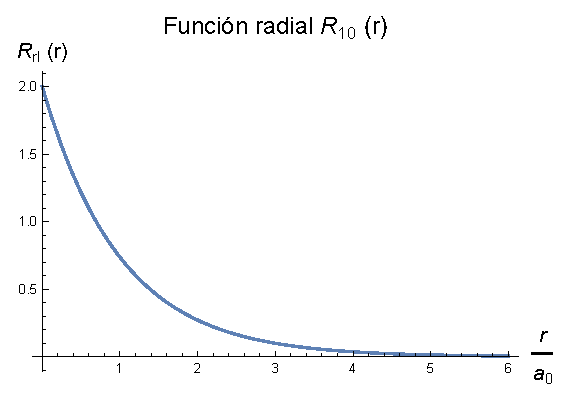
\includegraphics[scale=1]{Imagenes/Plot_Funcion_Radial_Hidrogeno_10_01.eps}
\end{figure}
\end{frame}
\begin{frame}
\frametitle{La función $R_{10} (r)$}
\begin{figure}
   \centering
   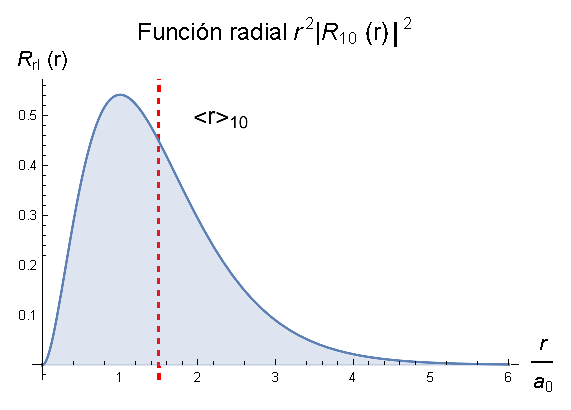
\includegraphics[scale=1]{Imagenes/Plot_Funcion_Radial_Hidrogeno_10_02.eps}
\end{figure}
\end{frame}
\begin{frame}
\frametitle{La función $R_{20} (r)$}
\begin{figure}
   \centering
   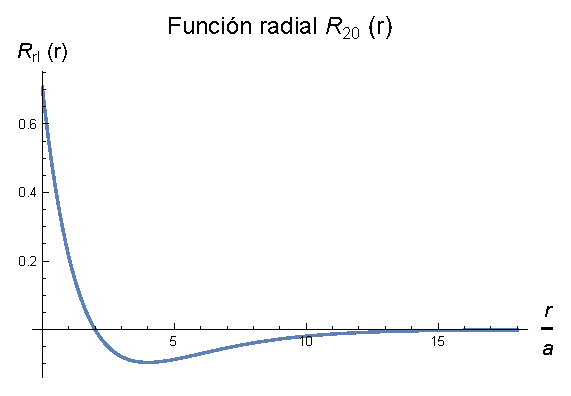
\includegraphics[scale=1]{Imagenes/Plot_Funcion_Radial_Hidrogeno_20_01.eps}
\end{figure}
\end{frame}
\begin{frame}
\frametitle{La función $R_{20} (r)$}
\begin{figure}
   \centering
   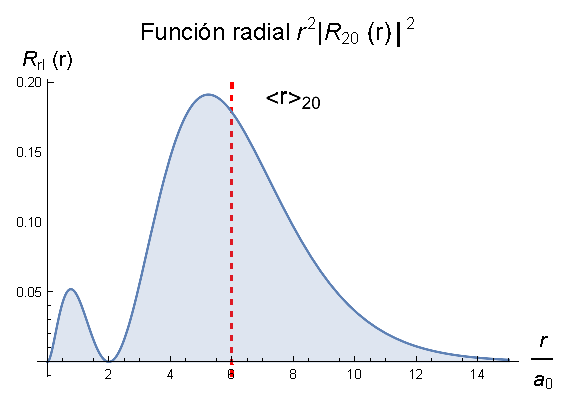
\includegraphics[scale=1]{Imagenes/Plot_Funcion_Radial_Hidrogeno_20_02.eps}
\end{figure}
\end{frame}
\begin{frame}
\frametitle{La función $R_{30} (r)$}
\begin{figure}
   \centering
   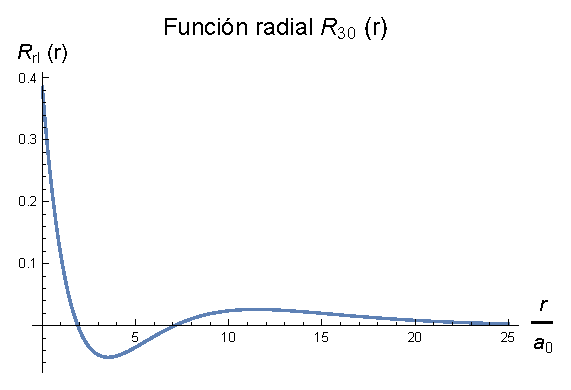
\includegraphics[scale=1]{Imagenes/Plot_Funcion_Radial_Hidrogeno_30_01.eps}
\end{figure}
\end{frame}
\begin{frame}
\frametitle{La función $R_{30} (r)$}
\begin{figure}
   \centering
   \includegraphics[scale=1]{Imagenes/Plot_Funcion_Radial_Hidrogeno_30_02.eps}
\end{figure}
\end{frame}
\begin{frame}
\frametitle{La función $R_{31} (r)$}
\begin{figure}
   \centering
   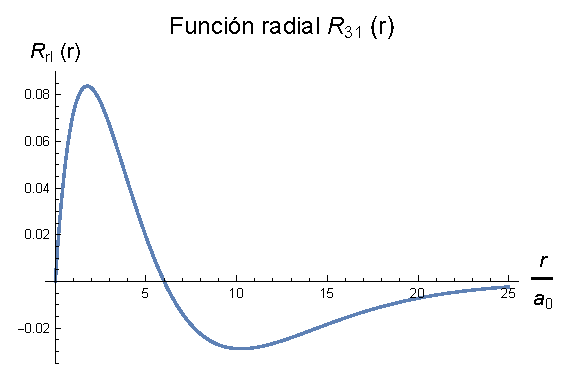
\includegraphics[scale=1]{Imagenes/Plot_Funcion_Radial_Hidrogeno_31_01.eps}
\end{figure}
\end{frame}
\begin{frame}
\frametitle{La función $R_{30} (r)$}
\begin{figure}
   \centering
   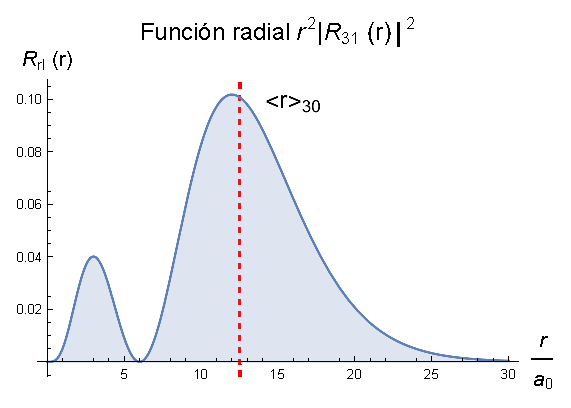
\includegraphics[scale=1]{Imagenes/Plot_Funcion_Radial_Hidrogeno_31_02.eps}
\end{figure}
\end{frame}
\begin{frame}
\frametitle{La función $R_{32} (r)$}
\begin{figure}
   \centering
   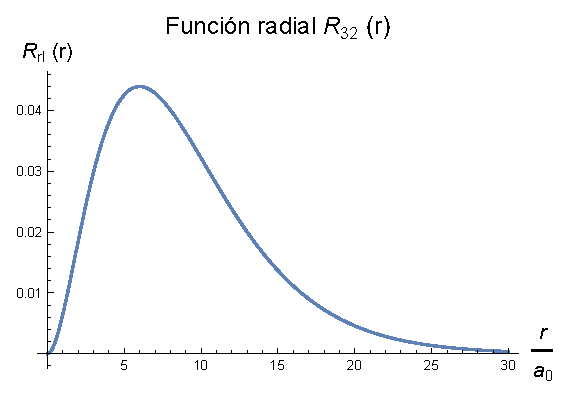
\includegraphics[scale=1]{Imagenes/Plot_Funcion_Radial_Hidrogeno_32_01.eps}
\end{figure}
\end{frame}
\begin{frame}
\frametitle{La función $R_{32} (r)$}
\begin{figure}
   \centering
   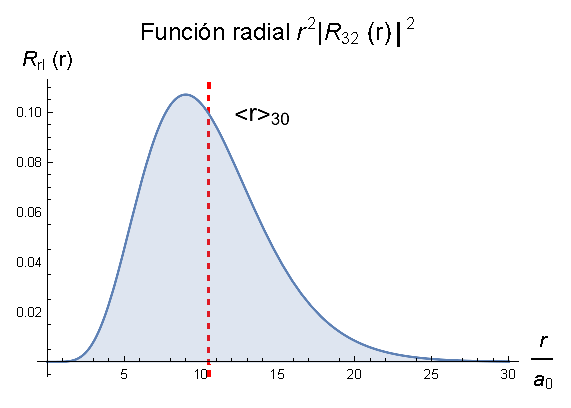
\includegraphics[scale=1]{Imagenes/Plot_Funcion_Radial_Hidrogeno_32_02.eps}
\end{figure}
\end{frame}
\begin{frame}
\frametitle{Sobre la densidad de probabilidad}
\setbeamercolor{item projected}{bg=black,fg=white}
\setbeamertemplate{enumerate items}{%
\usebeamercolor[bg]{item projected}%
\raisebox{1.5pt}{\colorbox{bg}{\color{fg}\footnotesize\insertenumlabel}}%
}
\begin{enumerate}[<+->]
\item $D_{n \ell} (0) = 0$ debido al término en $r^{2}$: \pause la densidad de probabilidad de encontrar el electrón es nula.
\seti
\end{enumerate}
\end{frame}
\begin{frame}
\frametitle{Sobre la densidad de probabilidad}
\setbeamercolor{item projected}{bg=black,fg=white}
\setbeamertemplate{enumerate items}{%
\usebeamercolor[bg]{item projected}%
\raisebox{1.5pt}{\colorbox{bg}{\color{fg}\footnotesize\insertenumlabel}}%
}
\begin{enumerate}[<+->]
\conti
\item $D_{n \ell} (r \to \infty) = 0$ \pause pues domina el término exponencial de $R_{n \ell} (r)$.
\seti
\end{enumerate}
\end{frame}
\begin{frame}
\frametitle{Sobre la densidad de probabilidad}
\setbeamercolor{item projected}{bg=black,fg=white}
\setbeamertemplate{enumerate items}{%
\usebeamercolor[bg]{item projected}%
\raisebox{1.5pt}{\colorbox{bg}{\color{fg}\footnotesize\insertenumlabel}}%
}
\begin{enumerate}[<+->]
\conti
\item $D_{n \ell} (r)$ se hace máxima para ciertos valores de $r$.
\\
\bigskip
\pause
En particular, se puede demostrar que:
\begin{align*}
r_{\max} (D_{n, \ell=n-1}) = n^{2} \, a_{0}
\end{align*}
\pause
De manera que el radio de Bohr da la posición del máximo para la densidad de probabilidad radial para el orbital con $\ell = \ell_{\max} = n - 1$
\end{enumerate}
\end{frame}
\begin{frame}
\frametitle{De la normalización}
De la condición de normalización, se cumple que:
\pause
\begin{align*}
\scaleint{6ex}_{\bs r=0}^{\infty} D_{n \ell} (r) \dd{r} = 1
\end{align*}
\end{frame}
\end{document}